\documentclass{article}
\usepackage[paperwidth=170mm,paperheight=89mm,margin=0mm]{geometry}
\usepackage[T1]{fontenc}
\usepackage{lmodern}
\usepackage{tikz}
\usetikzlibrary{arrows.meta}
\pagestyle{empty}
\setlength{\parindent}{0pt}
\definecolor{reference}{HTML}{147DA0}
\definecolor{testmodule}{HTML}{C66B32}
\definecolor{mcp}{HTML}{666879}
\begin{document}
\centering
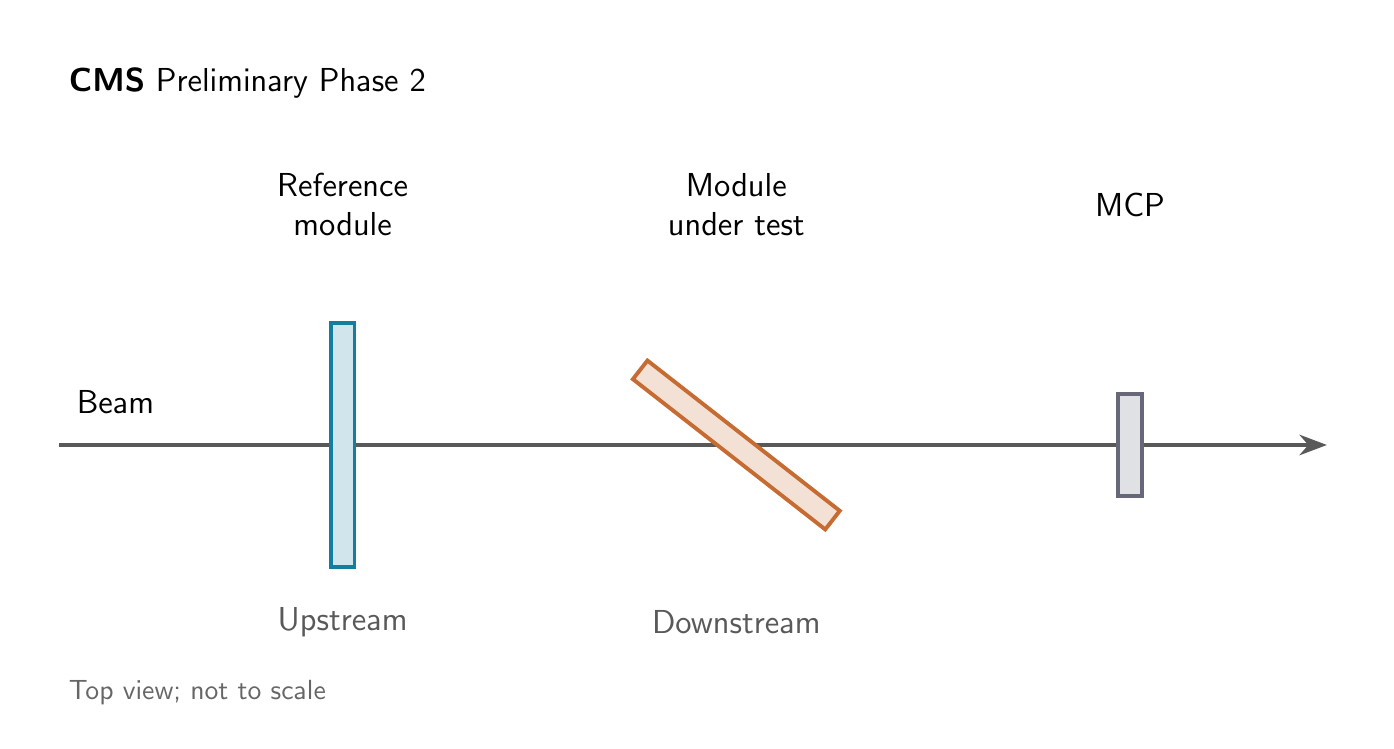
\begin{tikzpicture}[x=1cm,y=1cm,font=\sffamily\large]
  \path[use as bounding box] (0,0) rectangle (17,8.8);
  \node[anchor=west] at (.4,8.1) {\textbf{CMS} Preliminary Phase 2};

  \draw[-{Stealth[length=3.5mm]},line width=1.1pt,black!65]
    (.4,3.5) -- (16.5,3.5);
  \node[anchor=west] at (.5,4.05) {Beam};

  \filldraw[fill=reference!20,draw=reference,line width=1.4pt]
    (3.85,1.95) rectangle (4.15,5.05);
  \node[align=center] at (4,6.55) {Reference\\module};
  \node[text=black!65] at (4,1.25) {Upstream};

  % Rotation is relative to the plane perpendicular to the beam.
  \begin{scope}[rotate around={52:(9,3.5)}]
    \filldraw[fill=testmodule!20,draw=testmodule,line width=1.4pt]
      (8.85,1.95) rectangle (9.15,5.05);
  \end{scope}
  \node[align=center] at (9,6.55) {Module\\under test};
  \node[text=black!65] at (9,1.25) {Downstream};

  \filldraw[fill=mcp!20,draw=mcp,line width=1.4pt]
    (13.85,2.85) rectangle (14.15,4.15);
  \node[align=center] at (14,6.55) {MCP};

  \node[anchor=west,text=black!60,font=\sffamily\normalsize]
    at (.4,.35) {Top view; not to scale};
\end{tikzpicture}
\end{document}
